\section*{Question 2}

{\bfseries 2:Which is the effect when using the peak threshold=0.01 on the
'roofs1' image? Comment the differences with respect to the previous result.}

The peak threshold filters out keypoints whose extrema in the difference of Gaussian scale space are below a certain value. Increasing this threshold above the default value of 0 will effectively remove keypoints that lie in low contrast areas. This can be seen in figure \ref{fig:diff_peak_thresh}.

\begin{figure}[!hbt]
  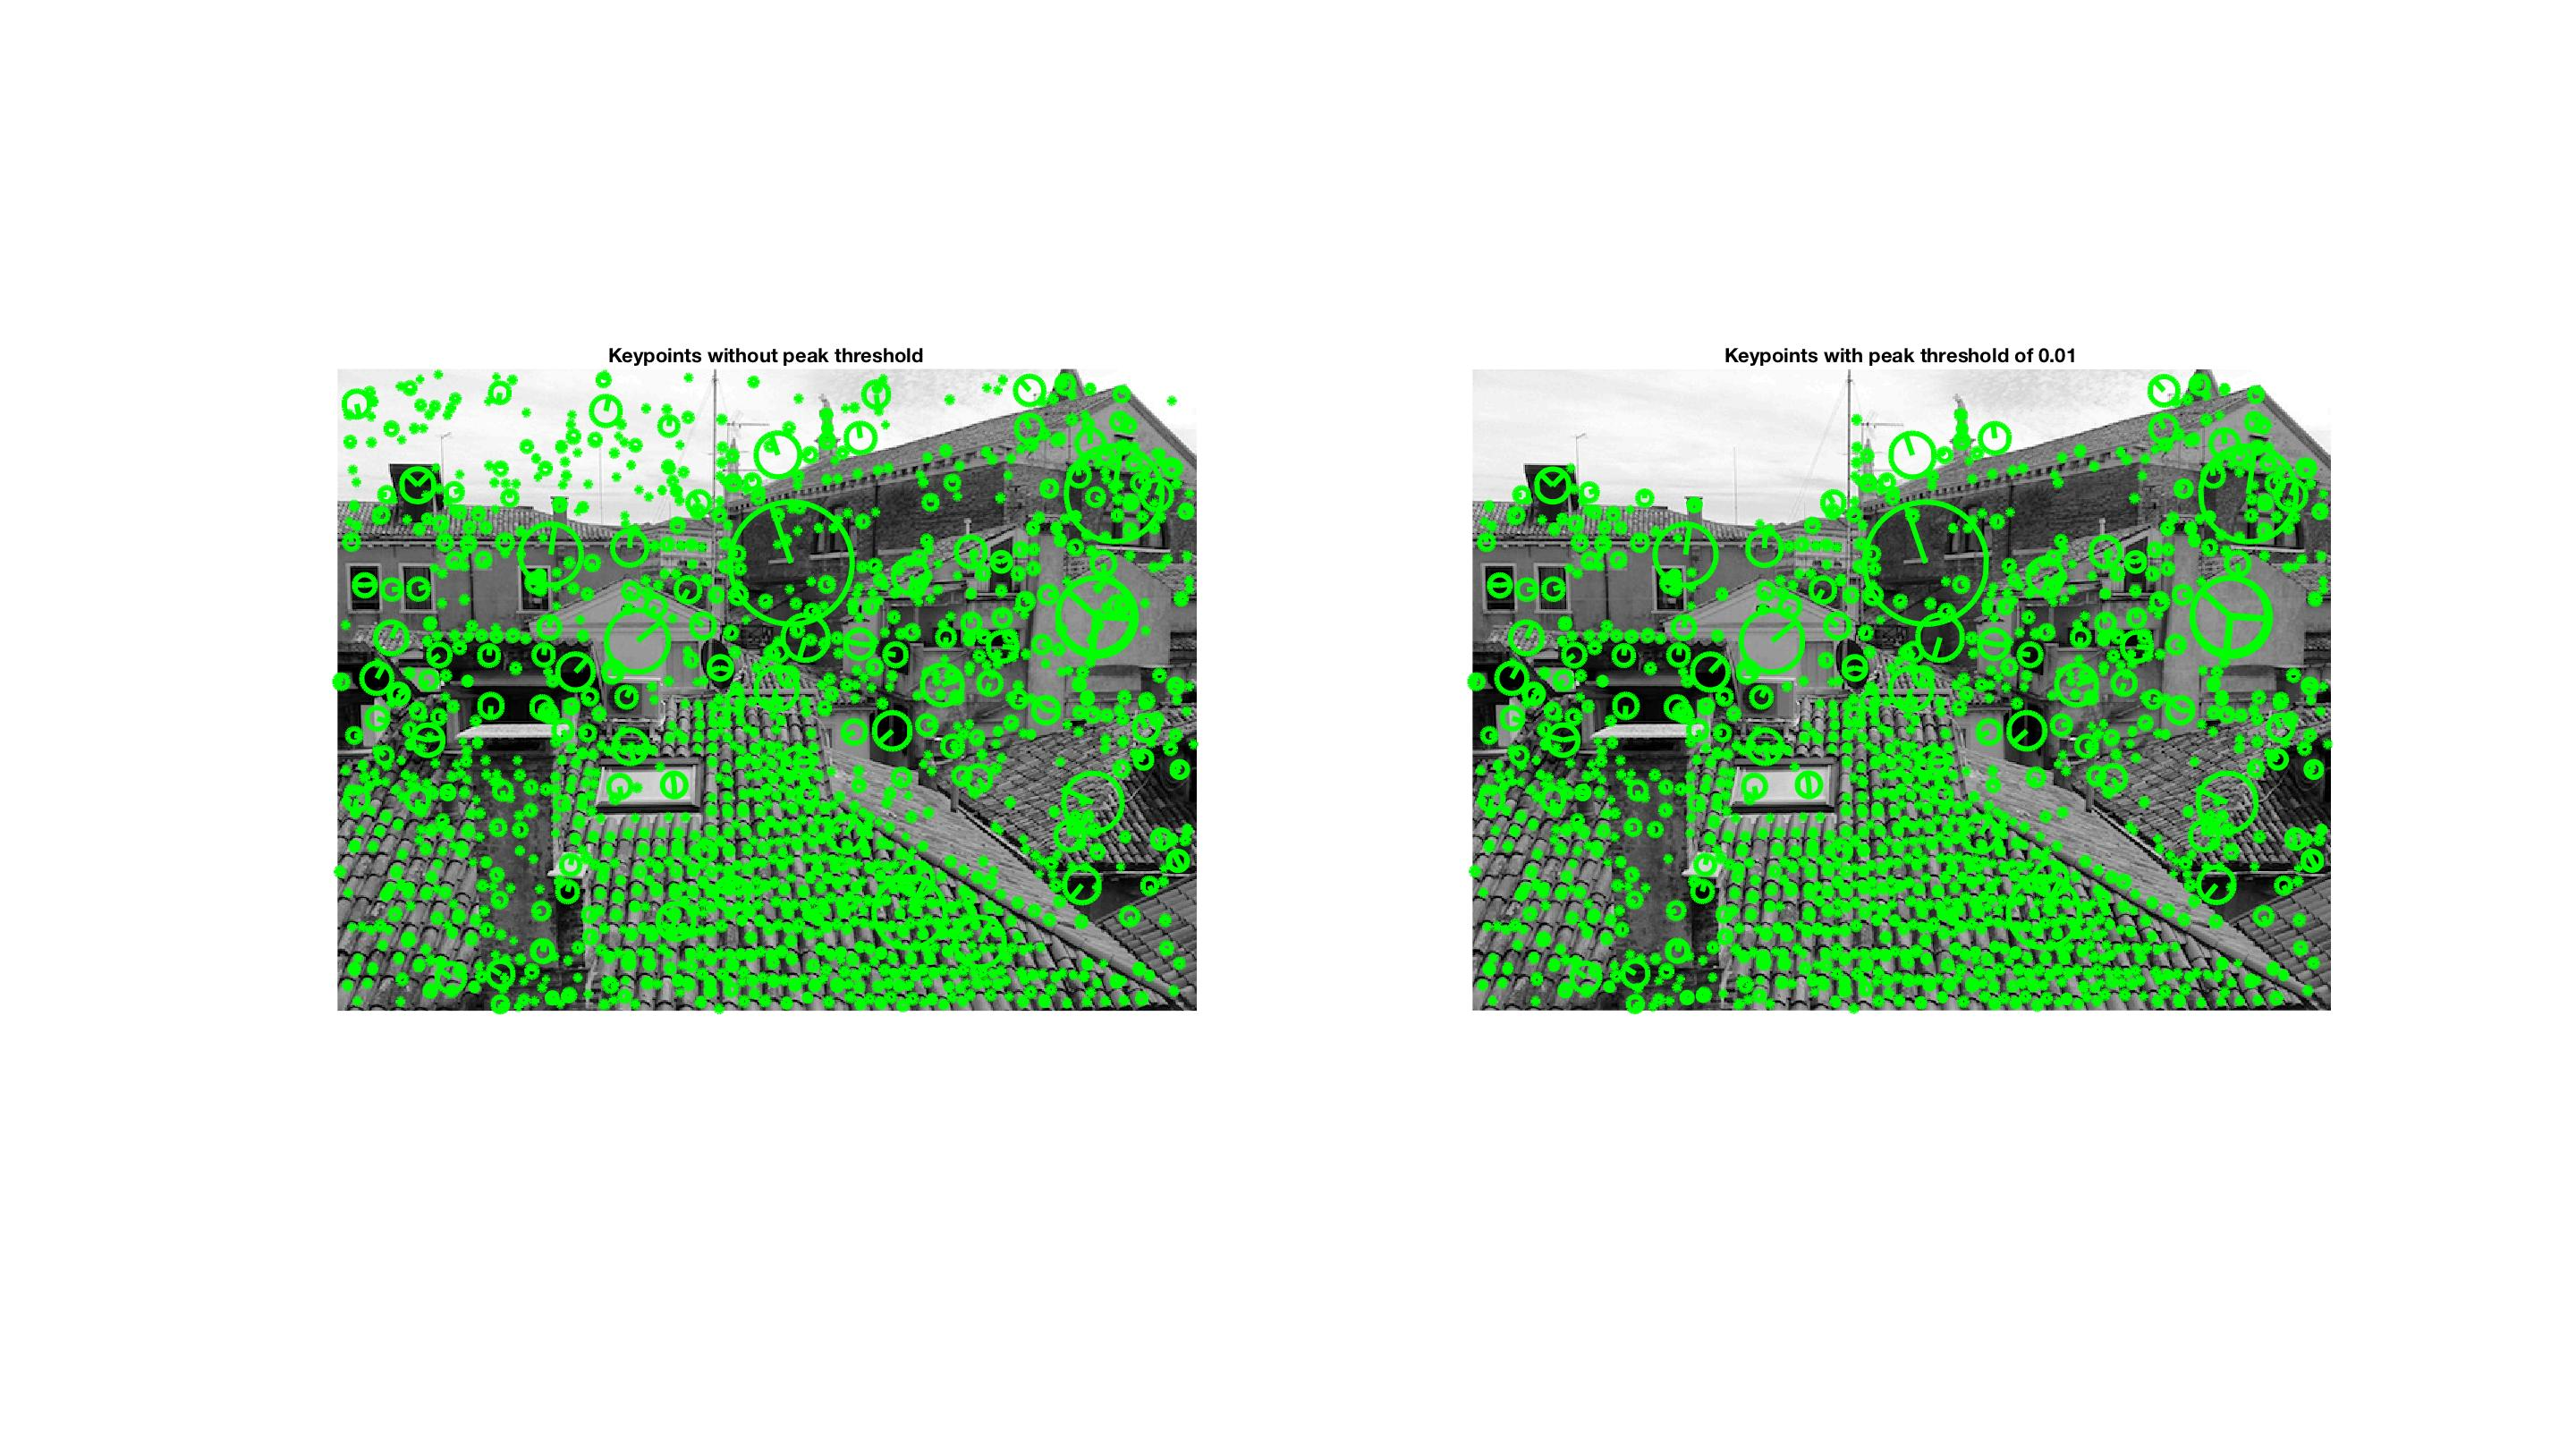
\includegraphics[width=\textwidth]{img/diff_peak_thresh}
  \caption{Comparison of peak threshold effects}
  \label{fig:diff_peak_thresh}
\end{figure}

As can be seen in figure \ref{fig:diff_peak_thresh}, the keypoints located on the comparatively low-contrast sky will be filtered out by the threshold of 0.01. Figure \ref{fig:diff_peak_thresh2} shows a zoomed in area in which the difference is notable the most.

\begin{figure}[!hbt]
  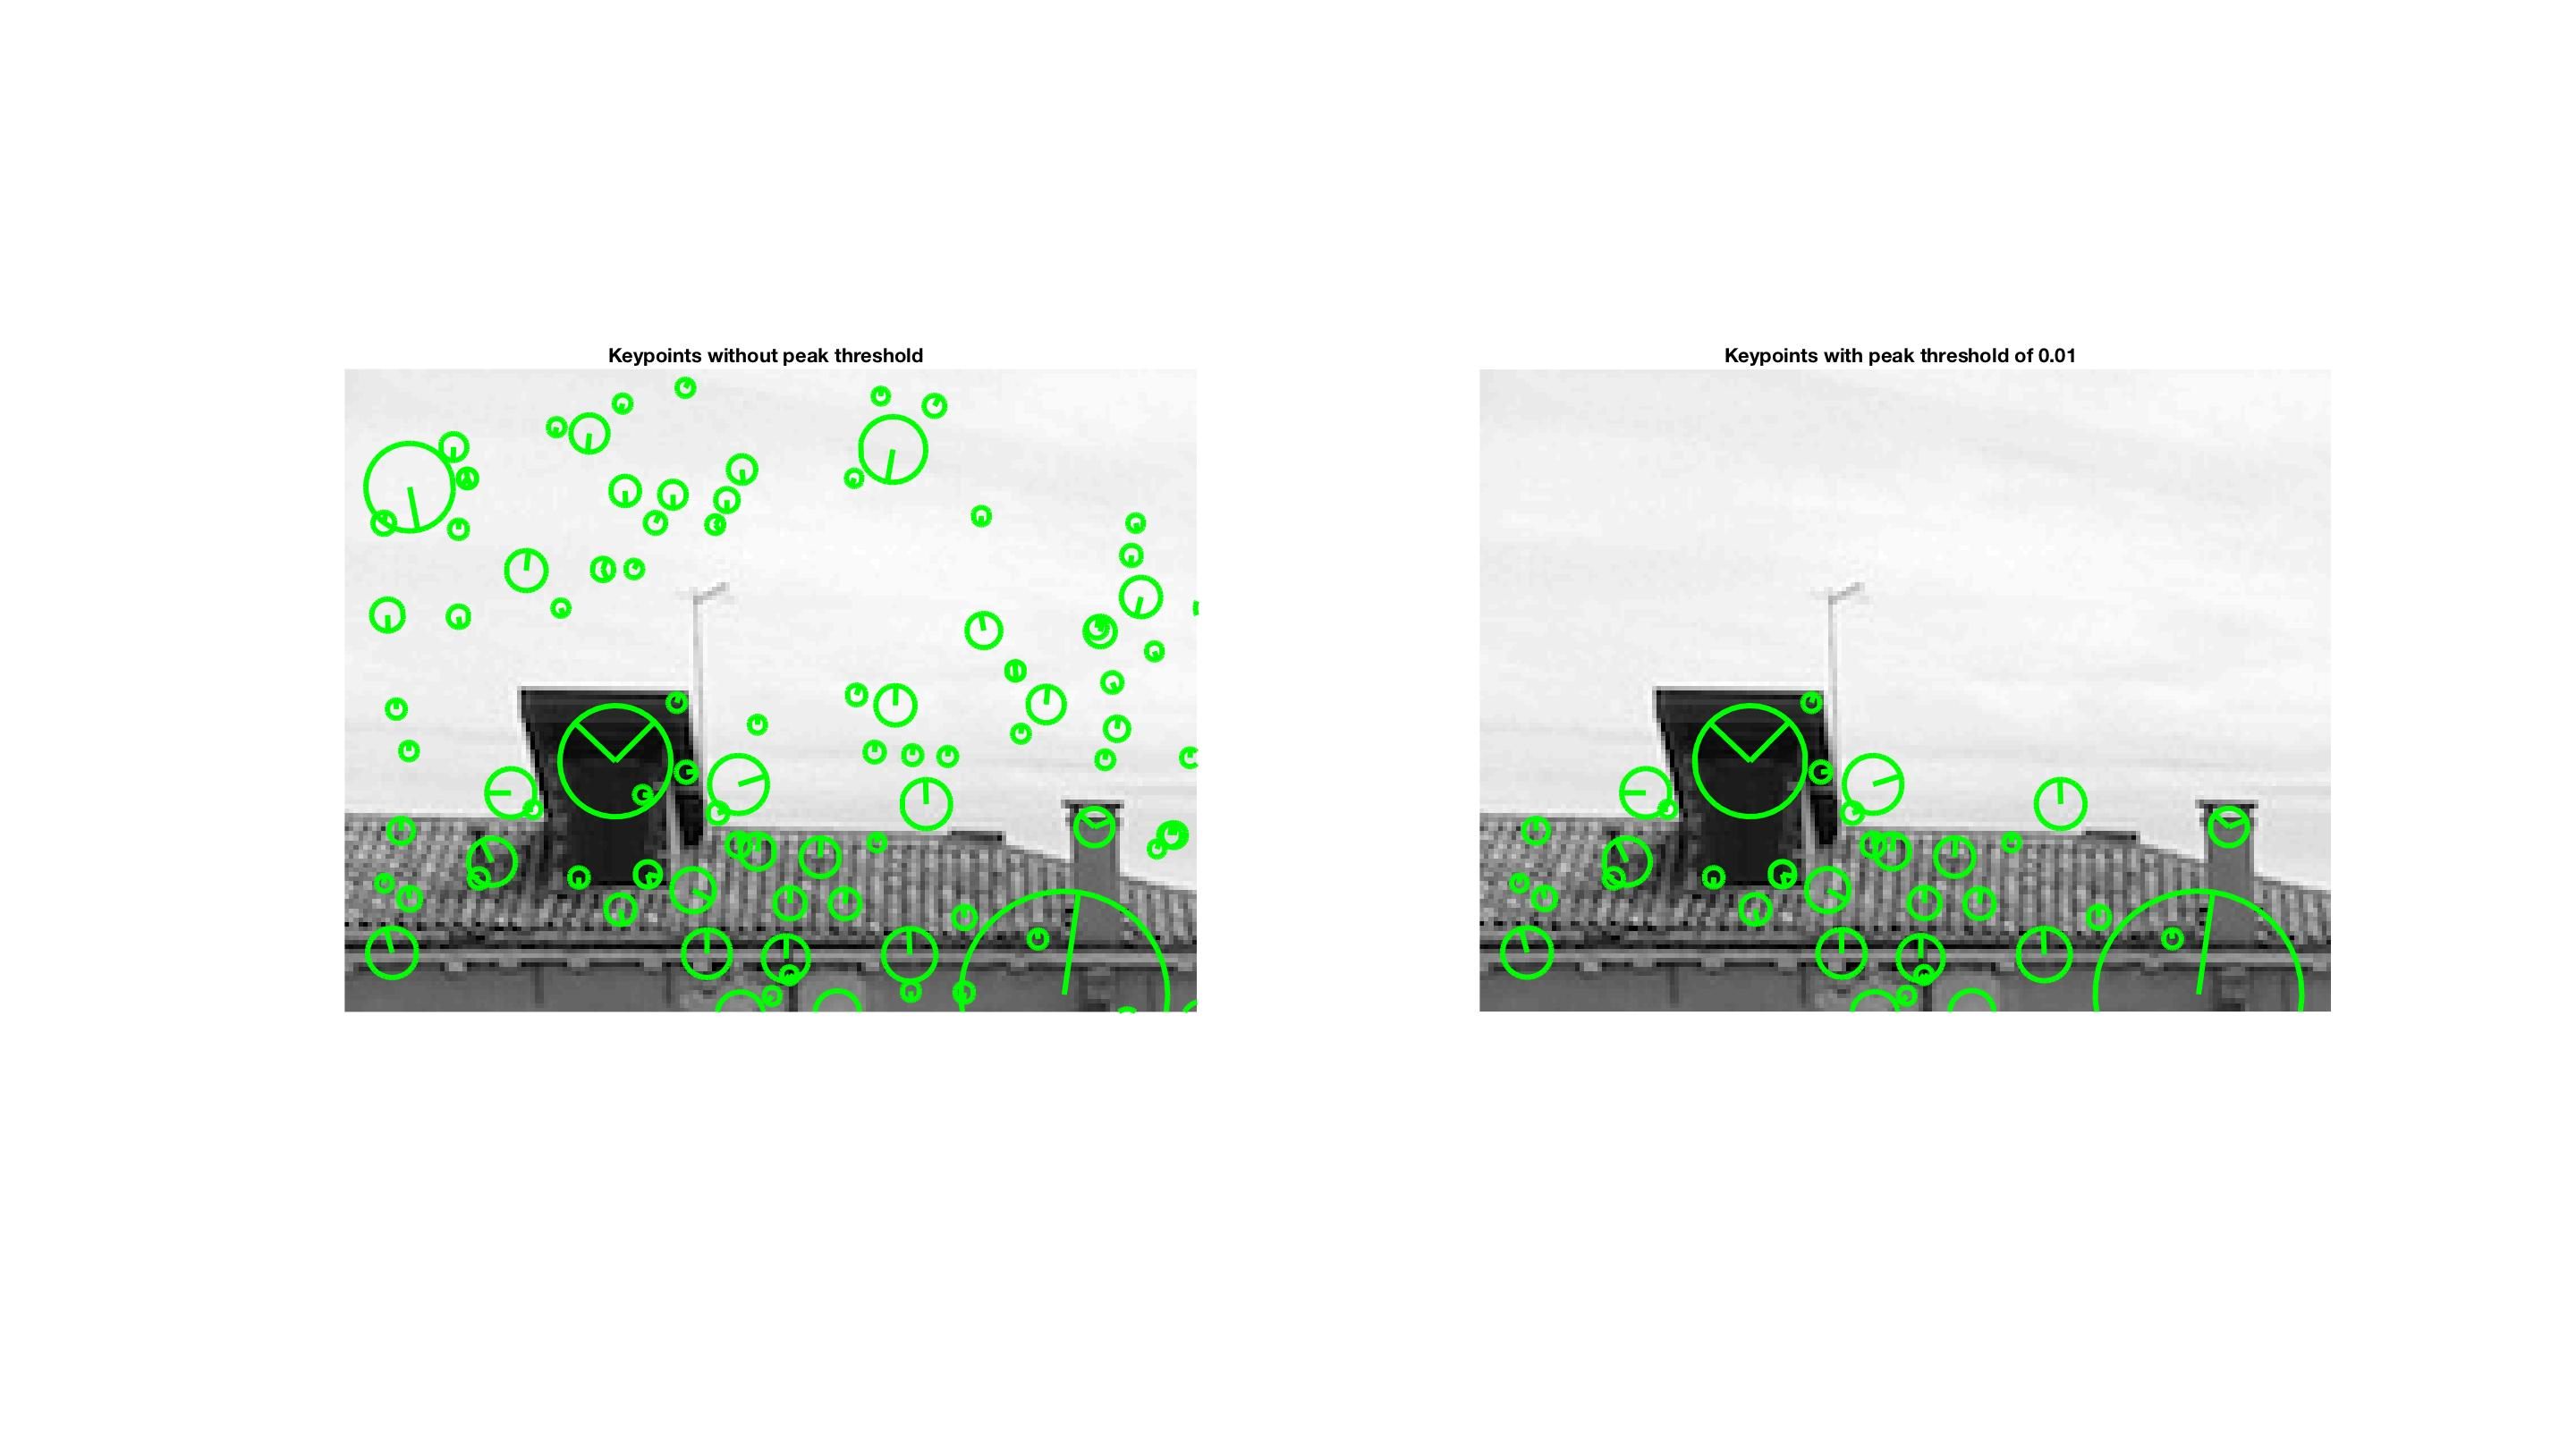
\includegraphics[width=\textwidth]{img/diff_peak_thresh2}
  \caption{Detailed comparison of peak threshold effects}
  \label{fig:diff_peak_thresh2}
\end{figure}

